\section{SVM}

\subsection[short]{Preparing the datas}

One of the first thing we noticed in the exploratory data analysis was that the target classes are unbalanced (\autoref{fig:target}). Indeed, among the $195$ observations, we had $48$ healthy people and $147$ people having the parkinson disease. This is roughly a $3:1$ ratio. Having unbalanced classes can be misleading as the algorithm could have "good score" even if it only predicts the majority class. 

In order to fix the imbalance, we upsampled the datas. The idea is to sample the datas with replacement by making multiple copy of observations belonging to the minority target class. The consequence is having a perfectly balanced dataset with $1:1$ target class ratio.

Next, we split the dataset into a training and testing test. We kept $30\%$ of the datas for testing purpose.

% TODO: speak about standardization

Plotting the datas for the training and testing sets on the two first principal components, we notice there is no trivial separation of the datas. The two first principal components accounts for roughly $64\%$ of the variation in the datas (respectively $46.8\%$ and $17.3\%$ for the first and second principal component) which is correct but not completely representative of the reality. However, we can already assume that a linear kernel will not be effective. Let's try it first though.

\begin{figure}[H]
	\centering
	\begin{subfigure}{0.49\textwidth}
		\centering
		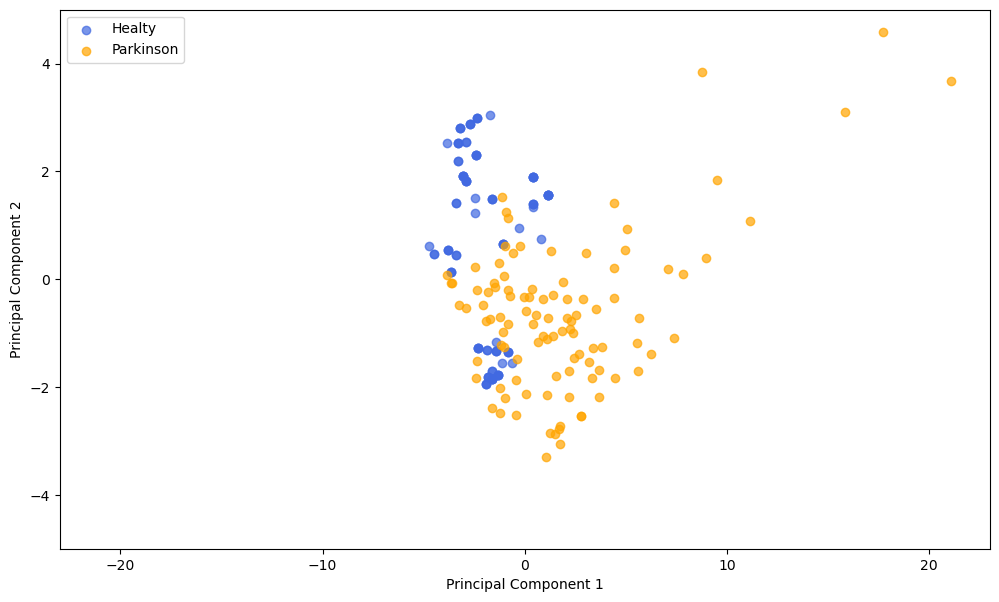
\includegraphics[width=\textwidth]{figures/plot_training_set.png}
		\label{fig:plot-training-set}
	\end{subfigure}
	\begin{subfigure}{0.49\textwidth}
		\centering
		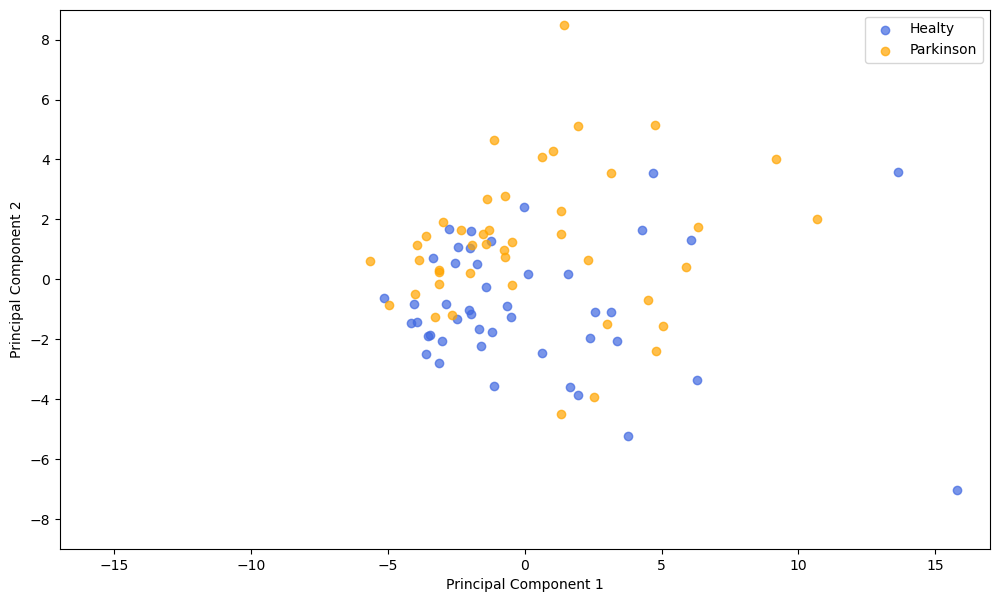
\includegraphics[width=\textwidth]{figures/plot_testing_set.png}
		\label{fig:plot-testing-set}
	\end{subfigure}
	\caption{Plot of the training set (at left) and testing set (at right) on the two first principal components.}
\end{figure}

\subsection[short]{Hard margin SVM}

We first try to find a separating hyperplane using a linear kernel.

Let $D = \set{(\vec{x}_i, \vec{y}_i)}_{i = 1}^{n}$ be our set of data points with $x_i \in \R^d$ (where \textit{d} is the dimension of the feature space) and $y_i \in \set{+1, -1}$.

Let $h: \R^d \rightarrow \R$, the equation of a plane defined $\forall x \in \R^d$ by, 
\begin{equation}
	h(\vec{x}) = \vec{w}^T \cdot \vec{x} + b
\end{equation}
where $\vec{w} \in \R^d$ is a vector of weights and $b$ is the bias.

A separating hyperplane is the set of points $\vec{x} \in \R^d$ that satisfy,
\begin{equation}
	h(\vec{x}) = 0
\end{equation}
such that we have $\forall \vec{x}_i \in D$ the following inequality,
\begin{equation} \label{eq:linear-constraint}
	y_i \cdot h(\vec{x}_i) \geq 1
\end{equation}

The hyperplane should yields the maximum margin among all possible separating hyperplanes, that is the parameters $\vec{w}$ and $b$ are the one that maximize $1 / ||\vec{w}||$.

An equivalent formulation is to say we want to minimize the following objective function,
\begin{equation}
	\min_{\vec{w}, b} {\frac{||\vec{w}||^2}{2}}
\end{equation}
subject to the linear constraint \autoref{eq:linear-constraint}.

The found hyperplane gets us an accuracy of $0.752$ on the testing set. However, a better way to assess the quality of a classifier is to look at the confusion matrix.

\begin{figure}[H]
	\centering
	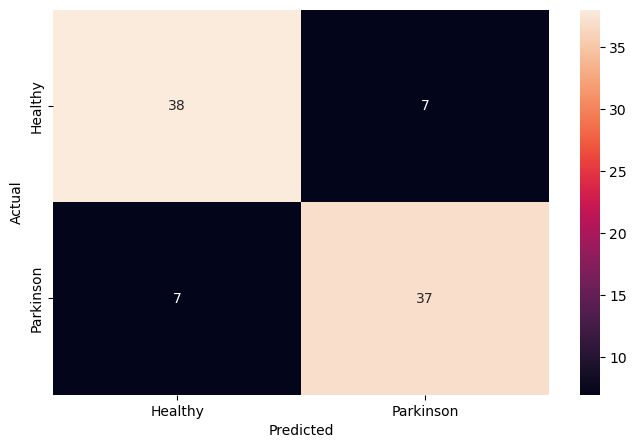
\includegraphics[width=0.5\textwidth]{figures/linear_svm_cm.png}
	\caption{Confusion matrix on the testing set for a linear SVM}
	\label{fig:linear-svm-cm}
\end{figure}

We notice that we have effectifely $\sim 25\%$ of missclassification. Therefore, we can conclude that a linear kernel is not ideal. On the following plot, we project the datas points of the training set on the two first principal components along with the support vectors. We also show the separating hyperplane and the margins. We have a confirmation of our first intuition, a linear kernel is not effective in separating these datas. 

\begin{figure}[H]
	\centering
	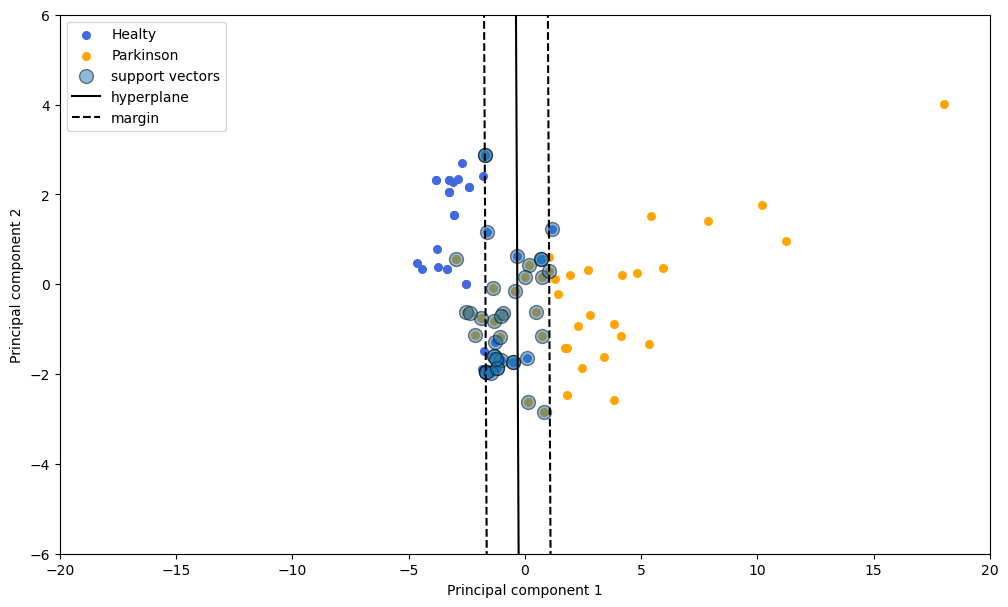
\includegraphics[width=0.7\textwidth]{figures/linear_svm_margins.png}
	\caption{Margins and separating hyperplane for a linear kernel SVM}
	\label{fig:linear-svm-margins}
\end{figure}

\subsection[short]{Hard margin SVM}

Despite the poor performance of the linear kernel. We can still try to improve it by introducing a \textit{slack variable} $\xi_i$, $i = 1,\dots,n$ that for each data point $x_i$ indicates how much it violates the separability condition\footnote{The separability condition ensures that the point is at least $\frac{1}{||\vec{w}||}$ from the hyperplane.}

$\forall \vec{x}_i \in D$ the inequality becomes,
\begin{equation} \label{eq:linear-constraint-xi}
	y_i \cdot h(\vec{x}_i) \geq 1 - \xi_i
\end{equation}

The goal is then to minimize the same objective function as before plus a penalty term,
\begin{equation}
	\min_{\vec{w}, b, \xi_i} {\frac{||\vec{w}||^2}{2}} - C \sum_{i=1}^{n} (x_i)^k
\end{equation}
where $C \in \R$ is a regularization constant and $k \in \R$.

This objective function is subject to the constraint above (\autoref{eq:linear-constraint-xi}) as well as $x_i \geq 0$ $\forall \vec{x}_i \in D$.

Performing a grid search with 5-fold cross-validation, we found an optimal regularization constant $C = 0.9$ giving a mean accuracy of $0.829$ on the validations sets and an accuracy of $0.753$ on the testing set. That is a slighlty better result than the hard margin case. Let's look at the confusion matrix,

\begin{figure}[H]
	\centering
	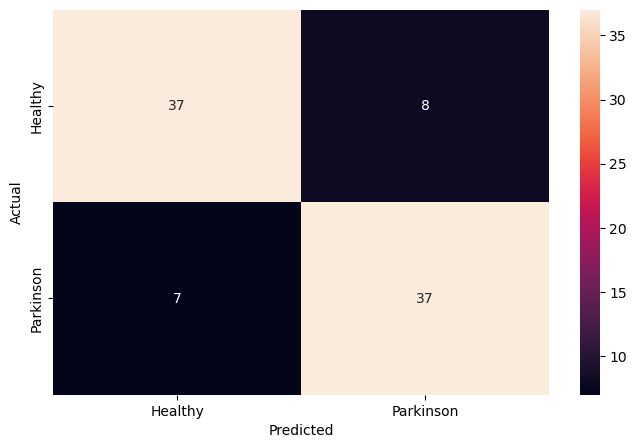
\includegraphics[width=0.5\textwidth]{figures/soft_svm_cm.png}
	\caption{Confusion matrix on the testing set for the soft margin case}
	\label{fig:soft-svm-cm}
\end{figure}

We notice that our classificer did not improve with the regularization parameters. So the linear classifier is definitely not helpful in separating these datas.

\subsection[short]{Kernel trick}

A to fix this problem is to map the data points in a high-dimension space by performing a non-linear transformation,
\begin{equation}
	\phi: \R^d \rightarrow \R^l, \quad \vec{x}_i \rightarrow \phi(\vec{x}_i)
\end{equation}

By this way, there is far more probability for the data to be linearly separable and because we perform a non-linear transformation, a linear separation in the feature space correspond to non linear decision region in the original data space.

We used a gaussian radial basis function for the kernel,
\begin{equation}
	\phi: \R^d \rightarrow \R^l, \quad \vec{x}_i \rightarrow \exp{\left( - (\gamma \vec{x}_i)^2 \right)}
\end{equation}
The kernel is then,
\begin{align}
	K(x_i, x_j) 
		&= \phi(x_i)^T \phi(x_j) \\
		&= \exp{\left( - \gamma (\vec{x}_i - \vec{x}_j)^2 \right)}
\end{align}

The $\gamma$ parameter has to be found by cross-validation. Performing a grid search on the $C$ and $\gamma$ parameters with a 5-fold cross-validation, we found the optimal parameters to be $C = 4.51$ and $\gamma = 0.005$. With these, we get a mean accuracy score of $0.961$ on the validation sets and an accuracy score of $0.888$ on the testing set. That's way better than using a linear kernel. We proove it by showing the confusion matrix, 

\begin{figure}[H]
	\centering
	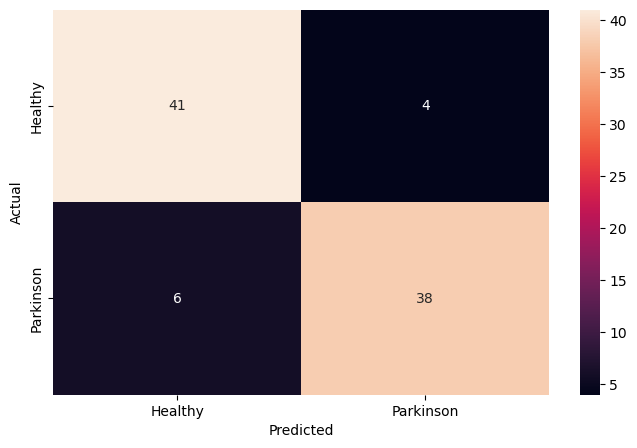
\includegraphics[width=0.5\textwidth]{figures/kernel_svm_cm.png}
	\caption{Confusion matrix on the testing set for a Gaussian kernel SVM}
	\label{fig:kernel-svm-cm}
\end{figure}

\begin{figure}[H]
	\centering
	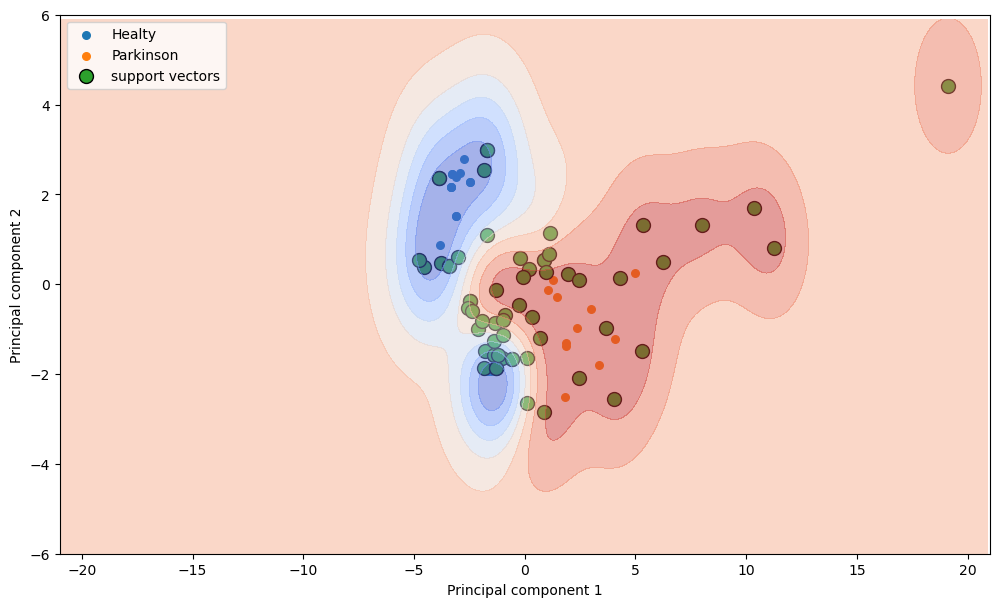
\includegraphics[width=0.7\textwidth]{figures/kernel_svm_region.png}
	\caption{Decision region for a Gaussian kernel SVM}
	\label{fig:kernel-svm-region}
\end{figure}
